%---------------------------------------------------------------------------------------------------
% Auswertung
%---------------------------------------------------------------------------------------------------
\section{Auswertung}\label{sec:auswertung}

Die Auswertung erfolgte anhand der ausgegebenen Graphen.
Wie in Abbildung~\ref{fig:speed_vs_height} und \ref{fig:acceleration_vs_height} zu sehen steigt die Fallgeschwindigkeit zunächst stark an.
Dabei ist das zu erreichende Maximum von der Absprunghöhe abhängig.
Liegt diese über einer Höhe von knapp $35000m$, überschreitet die Maximalgeschwindigkeit die lokale Schallgeschwindigkeit.

\begin{figure}[h]
  \centering
  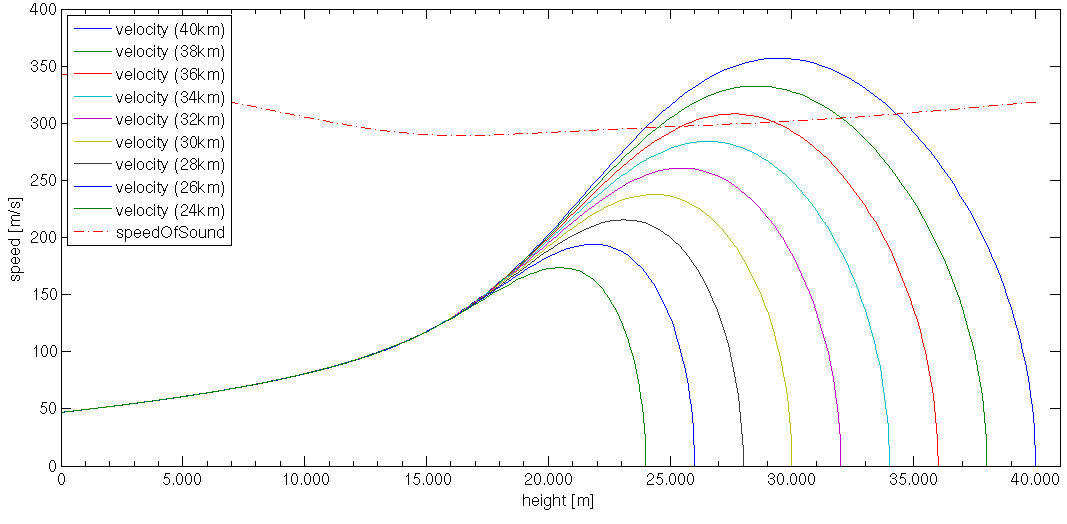
\includegraphics[width=1\textwidth]{speed_vs_height}
  \caption{Geschwindigkeit und Schallgeschwindigkeit, Sprünge 24-40km Höhe}
  \label{fig:speed_vs_height}
\end{figure}

\begin{figure}[h]
  \centering
  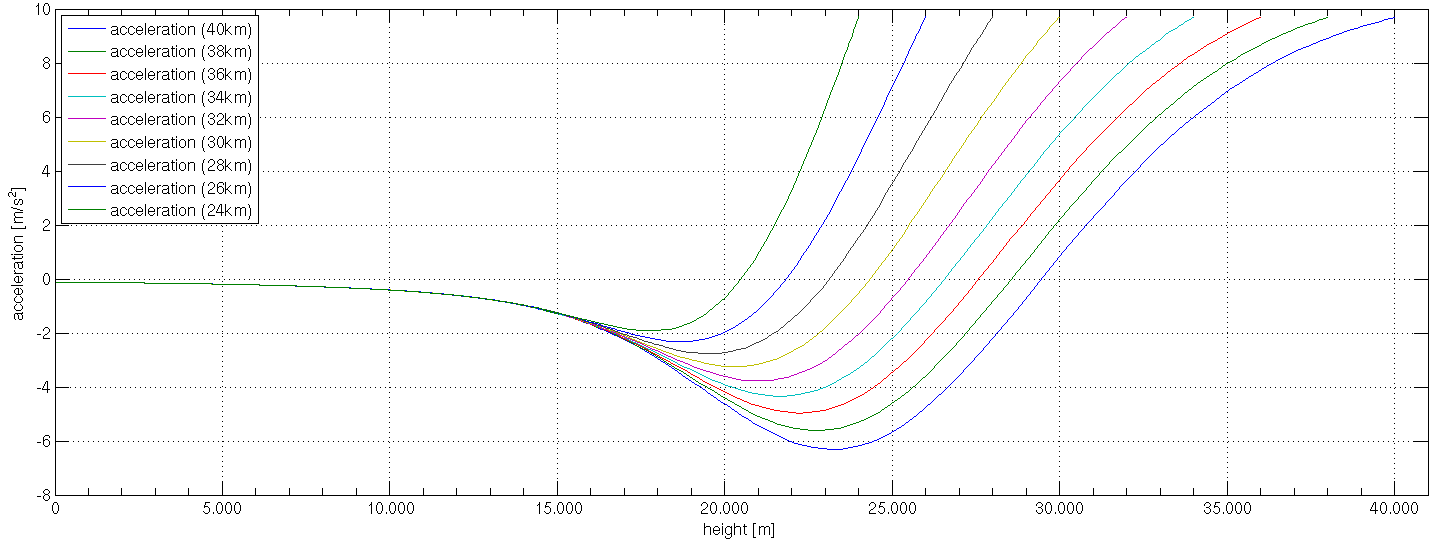
\includegraphics[width=1\textwidth]{acceleration_vs_height}
  \caption{Beschleunigung, Sprünge 24-40km Höhe}
  \label{fig:acceleration_vs_height}
\end{figure}

Unter der Annahme, dass für Joseph Kittinger im Jahre 1960 ähnliche Parameter galten, hat er bei seinem Sprung aus $31333m$ die Schallmauer nicht durchbrochen.
War dagegen der $c_w$-Wert günstiger, die angeströmte Fläche $A$ geringer oder die Absprungmasse $m_S$ größer könnte er es dennoch geschafft haben.

Die \textbf{nötige Absprunghöhe zum Durchbrechen der Schallmauer} liegt mit den gewählten Parametern bei $35240m$.

Weiterhin ist zu beobachten, dass sich die Geschwindigkeit unabhängig von der Absprunghöhe ab einer Höhe von ca. $15km$ bei allen Sprüngen gleich entwickelt.
Das \textbf{Auftreffen auf der Erdoberfläche} erfolgt bei allen simulierten Sprüngen mit einer Geschwindigkeit von knapp $47m/s$ oder knapp $170km/h$.
